\subsection{Fase 1}
Prima di tutto è stato determinato l'equivalente in acqua del calorimetro $M_e$. Questo processo è stato svolto già in un'altra esperienza quindi non è stato ripetuto. A causa di problematiche tecniche riscontrate durante l'utilizzo dell'apparato sperimentale, non è stato possibile impiegare i dati originariamente acquisiti nella precedente esperienza di laboratorio. Per proseguire con l'analisi, sono stati quindi utilizzati dati forniti dalla docente, rappresentativi di una situazione sperimentale reale.

\subsection{Fase 2}
In questa fase è stato svolo l'esperimento vero e proprio. Il calorimetro è stato riempito della stessa quantità d'acqua distillata $M$ con cui è stato misurato l'equivalente in acqua del calorimetro. Fatto ciò, il calorimetro è stato chiuso utilizzando un coperchio a cui sono stati fissati due resistori. È stato poi assemblato il circuito come in Figura (1).

\begin{figure}[H]
	\centering
	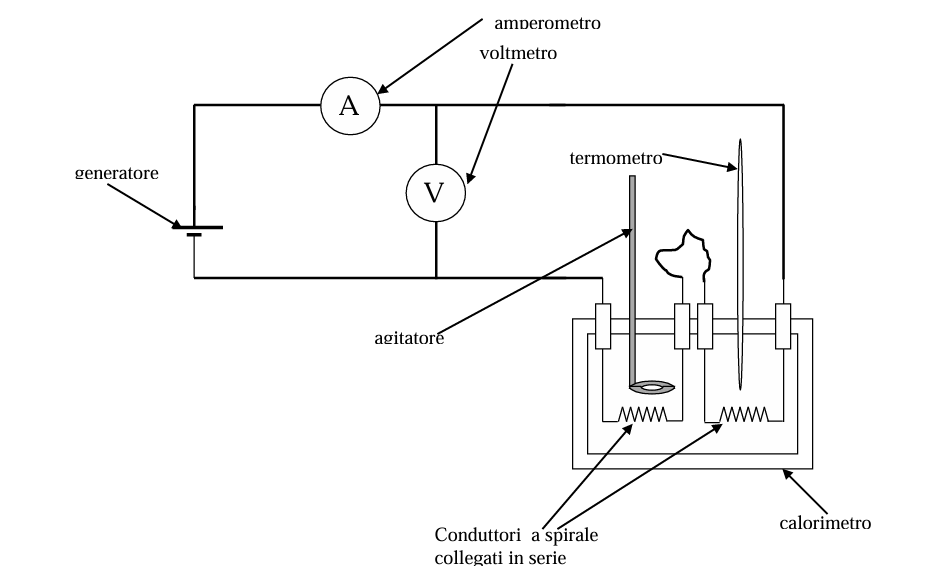
\includegraphics[width=0.70\textwidth]{./figures/Circuito}
	\caption{I due resistori sono stati connessi in serie al generatore di tensione. L'amperometro è stato posto in serie ai due resistori e il voltmetro in parallelo ad entrambi.}
\end{figure}

Utilizzando il voltmetro è stato possibile fissare la tensione del generatore a $5\ V$ e con l'amperometro è stata misurata la corrente circolante corrispondente. Dopo aver misurato la temperatura iniziale dell'acqua $T_0$, il generatore è stato acceso per dieci minuti. In questo lasso di tempo è stata misurata la temperatura dell'acqua ogni minuto. Coi dati raccolti è stato possibile misurare i valori di $E$ e $Q$